\documentclass{isistechreport}
\usepackage{booktabs}
\usepackage{array}
\usepackage{graphicx}
\usepackage{hyperref}
\usepackage{longtable}
\usepackage{tikz}
\usetikzlibrary{arrows.meta,positioning,fit,shapes.geometric}
\newcolumntype{L}[1]{>{\raggedright\arraybackslash}p{#1}}

\title{PyPTC: A User Guide to the Standalone Python Interface for PTC}
\author{Draft for code, physics, and reader review\\ISIS Neutron and Muon Source, Rutherford Appleton Laboratory}
\documentlabel{ISIS Technical Note --- DRAFT}
\email{Review status: pending}
\keywords{ISIS RCS, PyPTC, PTC, Python interface, tracking, optics}
\date{30 October 2026}

\begin{document}
\maketitle
\begin{abstract}
This draft documents the standalone PyPTC Python interface in this repository. It follows the user path from building the shared library and selecting a lattice to querying optics, tracking particles, applying apertures and errors, and inspecting outputs. It distinguishes code behavior from accelerator-physics interpretation and from functions available in the underlying PTC library but not exposed by PyPTC. Claims are tied to a frozen source revision; code correspondence, physics interpretation, and reader usefulness remain pending human review.
\end{abstract}
\tableofcontents
\clearpage

\section{Introduction and scope}
\label{sec:introduction}

PyPTC is the Python interface in this repository to a standalone PTC shared library. This note explains what a user can invoke through the Python package and how those calls reach the library. It is a guide to this implementation snapshot; it is not a general PTC manual, a MAD-X command guide, or a statement of ISIS operating policy. [claim:API-01]

PTC literature describes a broader polymorphic tracking and map-analysis system, including real and Taylor arithmetic and geometric lattice structures \cite{ForestSchmidtMcIntosh2002}. That context explains the lineage of the underlying code, but it does not prove that a feature is available in PyPTC. The exposed Python names, ABI symbols, and explicit unsupported-feature guards define the interface documented here. [claim:LIT-01]

The evidence basis is PyPTC commit \texttt{8824003c956390e921a1d469f77c247859a63258}; hashes and source roles are in \path{provenance/SOURCE_MANIFEST.csv}. This is an unreviewed draft. Physics meanings, sign conventions, operational suitability, and numerical acceptance criteria are not approved by this document. [claim:PROV-01]

\subsection{How to read evidence labels}

Claims tagged \texttt{implemented} describe behavior visible in the frozen source. \texttt{derived} claims report a named computation or execution. \texttt{domain\_interpretation} requires a domain authority and physics review. \texttt{unresolved} marks details not established by available evidence. The claim ledger in \path{provenance/CLAIMS.toml} records source symbols, line ranges, hashes, checks, and review status. [claim:PROV-02]

\subsection{PTC literature in context}

The original PTC report introduces PTC's symplectic-integrator, polymorphic Taylor, and fibre-bundle concepts \cite{ForestSchmidtMcIntosh2002}. Forest and Schmidt's PTC User's Reference Manual describes state, geometry, and tracking routines \cite{ForestSchmidtPTCManual2010}. Later author papers describe FPP and the MAD-X/PTC integration \cite{ForestNogiwaSchmidt2006FPPPTC,ForestNogiwaSchmidt2006FPPDoc,Schmidt2005MADXPTC,SkowronskiSchmidtForest2007}. These sources provide context for the underlying library and other interfaces; they are not PyPTC conformance tests. See the curated narrative and access record in \path{../literature_review.md}. [claim:LIT-01]

\section{Quick start}
\label{sec:quick-start}

\begin{center}
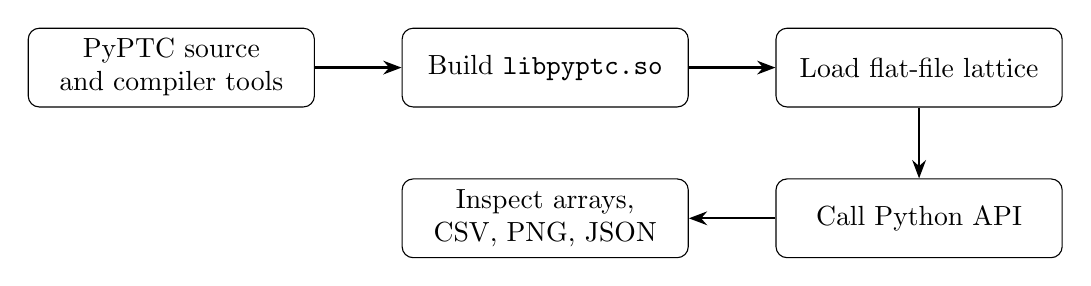
\begin{tikzpicture}[node distance=9mm and 11mm, box/.style={draw,rounded corners,align=center,text width=34mm,minimum height=10mm}, arr/.style={-{Stealth},thick}]
\node[box] (src) {PyPTC source and compiler tools};
\node[box,right=of src] (build) {Build \texttt{libpyptc.so}};
\node[box,right=of build] (lattice) {Load flat-file lattice};
\node[box,below=of lattice] (api) {Call Python API};
\node[box,left=of api] (result) {Inspect arrays, CSV, PNG, JSON};
\draw[arr] (src)--(build); \draw[arr] (build)--(lattice); \draw[arr] (lattice)--(api); \draw[arr] (api)--(result);
\end{tikzpicture}
\end{center}
The diagram summarizes the source-level user path; each box is described in the sections that follow. [claim:API-01]

\subsection{Build and import}

From the repository root, run the documented local build command:
\begin{verbatim}
bash build/build_ptc.sh
python3 -c "from pyptc import PTC; print('PyPTC import OK')"
\end{verbatim}
The build script requires \texttt{meson} and \texttt{nm}, compiles the shared library under \texttt{build\_pyptc/}, checks exported symbols, and performs a ctypes load smoke check. A successful import alone does not establish that the lattice loads or that a physical calculation is validated. [claim:BUILD-01]

\subsection{Minimal lattice and optics call}

The default lattice constant resolves to the generated simplified flat file. A helper generates the file if it is absent, empty, or explicitly requested for regeneration. A legacy readiness file is separately named and is not the default. [claim:LATTICE-01]

\begin{verbatim}
from pyptc import PTC, DEFAULT_LATTICE

ptc = PTC()
ptc.init_lattice(DEFAULT_LATTICE)
ptc.update_twiss()
print(ptc.tunes())
rows = ptc.all_node_twiss_orbit()
print(f"rows: {len(rows)}")
\end{verbatim}
The method sequence is directly exposed in the Python wrapper. The exact numeric values depend on the selected lattice and build and should be recorded with those inputs. This excerpt is a starter workflow, not a tolerance or acceptance test. [claim:API-02]

\subsection{Expected output and next steps}

The plotting examples write user-facing files under \texttt{test\_outputs/}; the bare optics example writes a Twiss/orbit plot, CSV rows, and a JSON summary. The bunch example writes separate initial/final dashboards and diagnostic CSV products. Run the matching example script to regenerate outputs; copied figures in this note are frozen repository artifacts and are not generated during LaTeX compilation. [claim:EXAMPLE-01]

\begin{verbatim}
python3 examples/01_plot_bare_twiss_closed_orbit.py
python3 examples/02_track_bunch_dashboard.py
\end{verbatim}
For installation details, lattice generation inputs, and dependencies, follow the repository README and example-specific script. [claim:BUILD-01]

\section{User path through the package}
\label{sec:user-path}

The public package exports the \texttt{PTC} class, lattice helpers, parser record types, error/aperture readers, and diagnostic plotting helpers. The package is organized into API, lattice, aperture, error-table, bunch, and plotting modules. Its initializer identifies the exported subset; method behavior is traced to its defining module. [claim:API-01]

\begin{description}
  \item[Construct] \texttt{PTC(library=DEFAULT\_LIBRARY)} loads the configured shared library and checks that the file exists; a missing library raises \texttt{FileNotFoundError}. [claim:API-02]
  \item[Initialize] \texttt{init\_lattice(path)} stores a resolved lattice path and passes it to the PTC initialization symbol. \texttt{run\_script(path)} and \texttt{read\_accel\_table(path)} pass resolved file paths to corresponding library entry points. [claim:API-03]
  \item[Query] Methods such as \texttt{tunes()}, \texttt{chromaticities()}, and \texttt{node\_phase\_advances()} allocate Python/ctypes outputs, call ABI symbols, check status where provided, and return Python dictionaries or NumPy arrays. [claim:API-04]
  \item[Edit] Misalignment, aperture, error-table, and machine-control methods call dedicated C ABI functions from the Python wrapper. Their argument units and operational interpretation require review where not settled by code. [claim:API-05]
  \item[Track] The particle-tracking methods convert Python bunch rows into the six-value PTC coordinate array, call the ring tracking entry point, and convert final values back into the package convention. [claim:TRACK-01]
\end{description}

\subsection{Python, ABI, and parent PTC boundary}

The Python wrapper configures shared-library function signatures through \texttt{ctypes}. The companion \texttt{fortran/pyptc\_api.f90} contains the exposed shim implementations, which in turn call routines from the parent PTC code. The build script verifies a defined set of exported names. This note's feature claims stop at that inspected call chain; it does not provide a line-by-line account of the entire parent PTC source tree. [claim:ABI-01]

\subsection{Errors and failures}

The wrapper converts nonzero status values into \texttt{RuntimeError} through \texttt{\_check\_status}. Name-based fibre lookup requires an initialized or explicitly supplied lattice path; missing names and occurrences raise \texttt{ValueError}. Input shape guards reject particle coordinates that are not length six and bunch arrays that are not \texttt{N x 6}. [claim:FAIL-01]

\section{Public API map}
\label{sec:api-map}

This inventory follows the names a Python user can call. Methods beginning with an underscore are internal helpers and are omitted. The signatures in source remain authoritative; this summary groups methods by the interaction they support. Values and units are not inferred from names. [claim:API-06]

\begin{longtable}{L{0.31\textwidth}L{0.62\textwidth}}
\toprule
\textbf{User task} & \textbf{Methods} \\
\midrule
\endfirsthead
\toprule \textbf{User task} & \textbf{Methods} \\
\midrule
\endhead
Create/query context & \texttt{PTC(...)}; \texttt{api\_level()}, \texttt{init\_lattice()}, \texttt{run\_script()}, \texttt{read\_accel\_table()}, \texttt{update\_twiss()}, \texttt{machine\_summary()}, \texttt{scalar()} \\
Read optics/orbit & \texttt{tunes()}, \texttt{chromaticities()}, \texttt{node\_phase\_advances()}, \texttt{node\_twiss\_orbit()}, \texttt{all\_node\_twiss\_orbit()}, \texttt{task\_type()} \\
Track particles & \texttt{track\_particle\_ptc()}, \texttt{track\_particle\_ptc\_with\_loss()}, \texttt{track\_bunch()}, \texttt{track\_bunch\_with\_losses()}, \texttt{particle\_diagnostics()} \\
Edit alignment/errors & \texttt{set\_misalignment()}, \texttt{set\_madx\_misalignment()}, \texttt{add\_madx\_multipole\_error()}, name-based variants, \texttt{apply\_misalignments()}, \texttt{apply\_madx\_error\_table()} \\
Apply/query apertures & \texttt{set\_aperture()}, name-based set/get, \texttt{get\_aperture()}, \texttt{apply\_rectangular\_apertures()}, \texttt{apply\_madx\_aperture\_file()}, \texttt{all\_fibre\_apertures()}, disable methods, \texttt{absolute\_aperture()}, \texttt{set\_absolute\_aperture()} \\
Time-dependent controls & \texttt{set\_acceleration()}, \texttt{set\_ramping()}, \texttt{set\_modulation()}, \texttt{set\_cavity()}, orbit-state methods, \texttt{energize\_lattice()}, orbit-time methods, cavity setup/power/total-path methods, AC and ramp magnet configuration \\
\bottomrule
\end{longtable}

Module-level helpers include flat-file fibre parsing and name resolution; MAD-X aperture and error-table readers; JVT design aperture reader; matched Gaussian bunch helper; tune summary, CSV writers, and plotting helpers. The exported subset is listed in \path{pyptc/__init__.py}. Utility functions and source examples are not equivalent to one monolithic managed simulation workflow. [claim:API-01]

The time-dependent control group is present in the Python wrapper and ABI, but this guide does not assert a validated ramping, RF, or acceleration procedure for the ISIS RCS. Treat those methods as interface entry points pending a separately evidenced and physics-reviewed workflow. [claim:CONTROL-01]

\section{Lattice and optics interaction}
\label{sec:optics}

The lattice helper parses PTC flat-file fibre blocks and exposes one-based fibre indices, element names, lengths, and source line spans. Name resolution first looks for an exact element-name match, then supports a parent dipole name expanding to numbered sliced dipole records. This is a parser contract for the flat-file form, not a general MAD-X sequence parser. [claim:LATTICE-02]

After lattice initialization and Twiss update, users can query tunes, chromaticities, phase advances, and per-node Twiss/orbit data through \texttt{PTC}. The code returns values and field names; physical coordinate meaning, unit conventions, and validity ranges are separate review questions. Do not infer them from names alone. [claim:API-04]

\begin{figure}[ht]
  \centering
  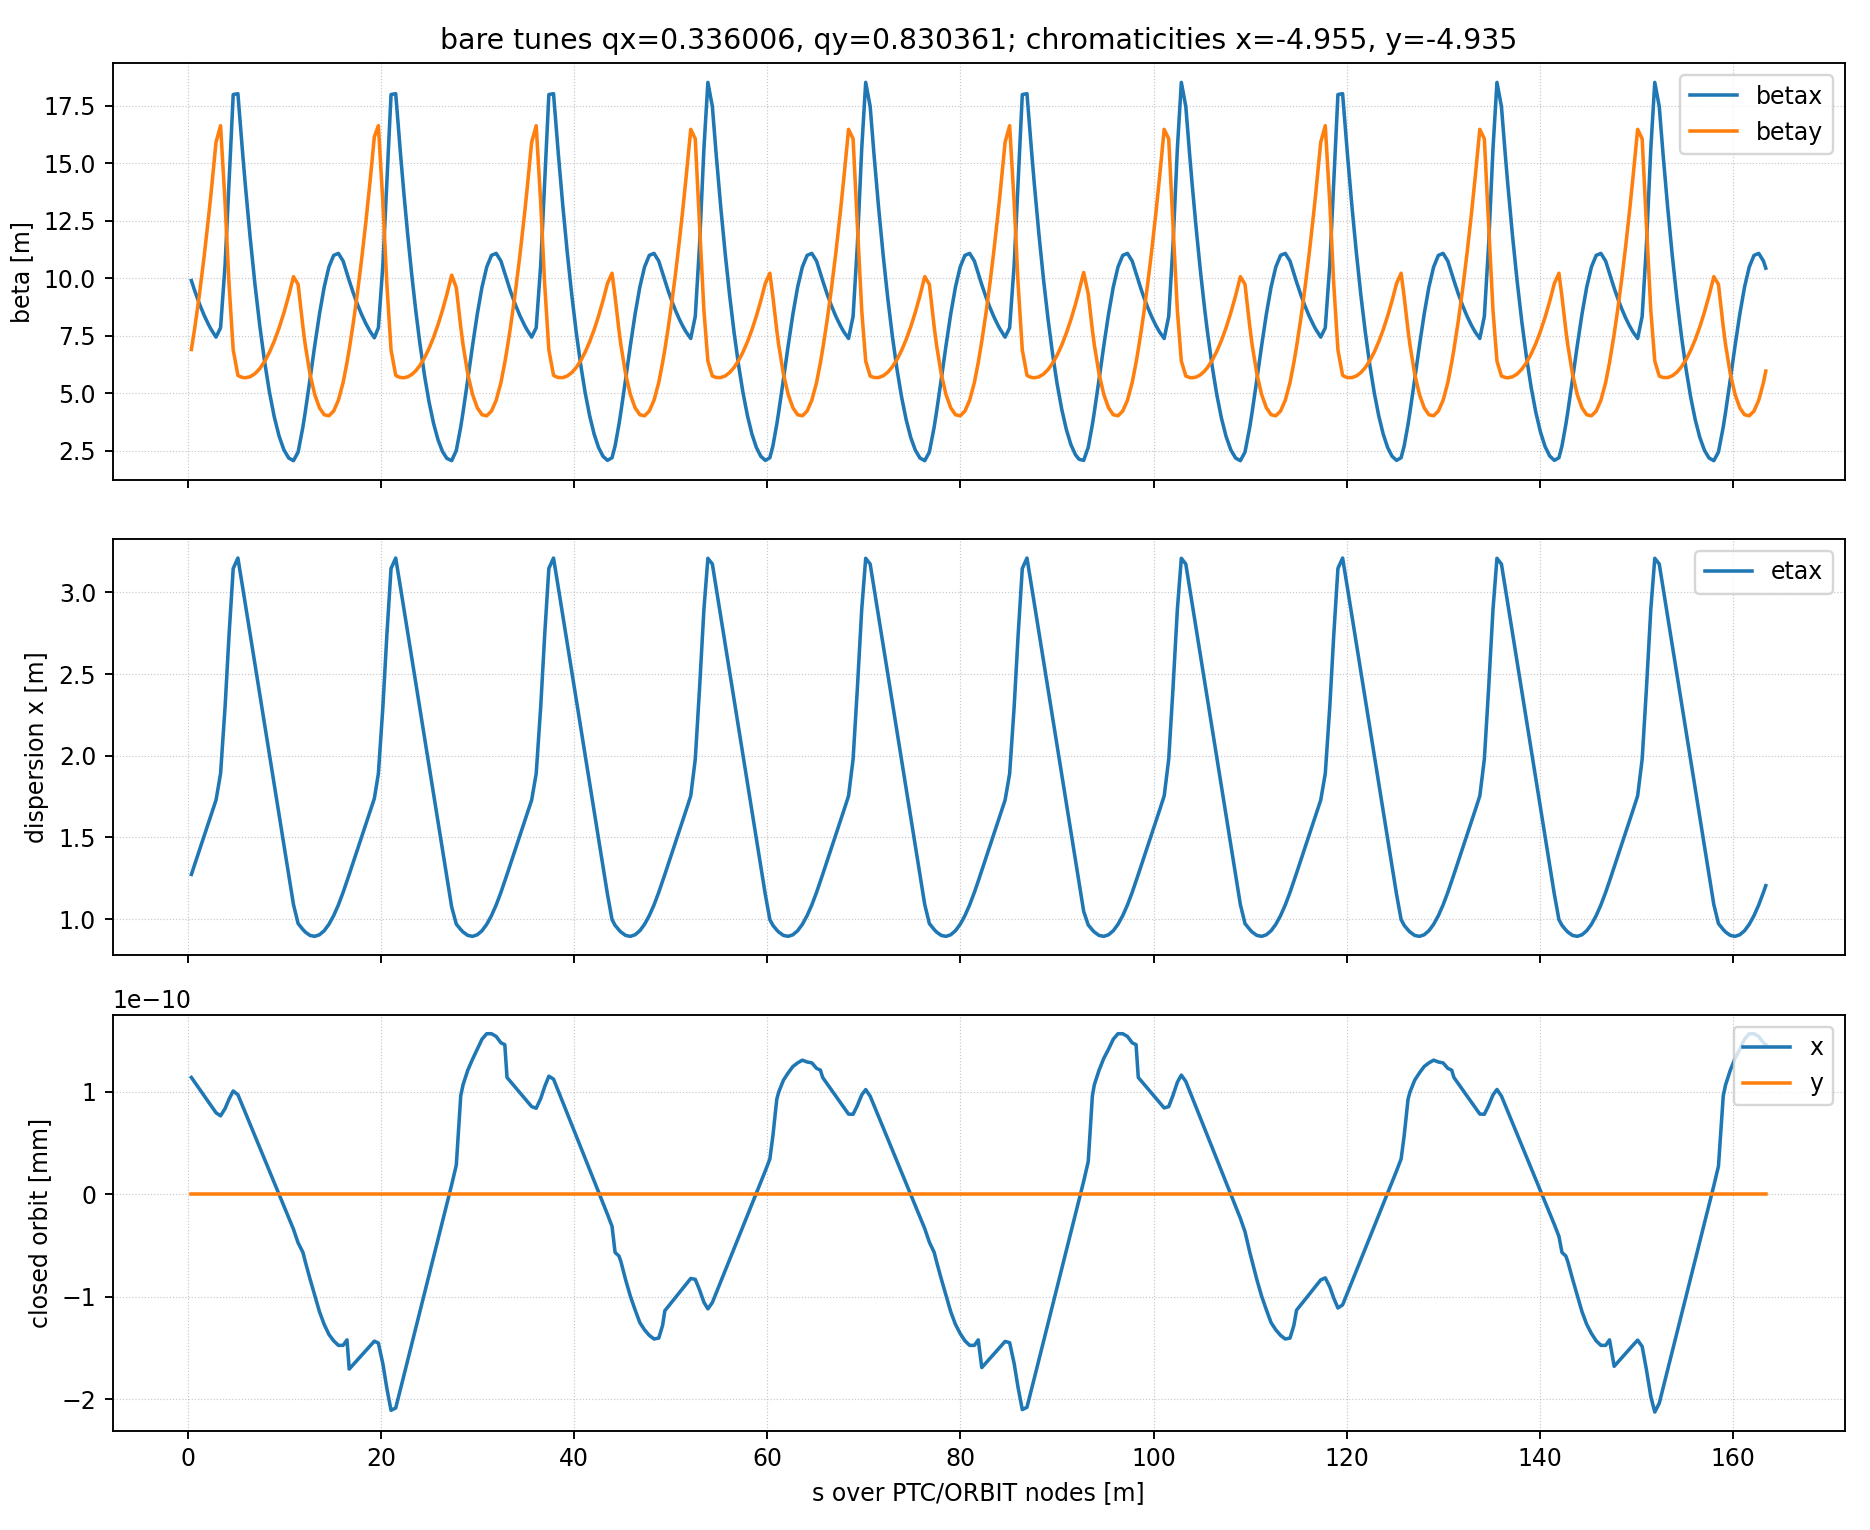
\includegraphics[width=0.96\textwidth]{figures/bare_twiss_closed_orbit.png}
  \caption{Repository optics diagnostic generated by the bare optics example. The copied pixels are unchanged. It illustrates the plotted fields available from this example; it is not a comparison to a reference model or physics acceptance. [claim:PROV-03]}
\end{figure}

\subsection{One-turn maps and normal forms}

\texttt{one\_turn\_map()} and \texttt{normal\_form()} both raise the not-exposed exception. [claim:LIMIT-01]

\section{Particle and bunch tracking}
\label{sec:tracking}

The bunch helpers accept rows in the Python/PyParticleBunch order \texttt{x, xp, y, yp, z, dE}; \texttt{dE} is a total-energy deviation. In the default PTC tracking state used by these helpers, the fifth coordinate is relative momentum deviation, \(\delta=p/p_0-1\), rather than relative energy deviation. With synchronous energy \(E_0=p_0c/\beta_0\) and inferred rest mass \(m^2=E_0^2-(p_0c)^2\), the wrapper computes \(\delta=\sqrt{(E_0+dE)^2-m^2}/p_0c-1\). The inverse is \(dE=\sqrt{m^2+[p_0c(1+\delta)]^2}-E_0\). The sixth-coordinate mapping is \(L=-z/\beta_0\). This documents the implemented convention and its code/manual basis; it is not a physics validation of every active PTC state or operating regime. [claim:TRACK-01] [claim:TRACK-02]

\path{track_bunch()} uses the same conversion at each node while updating the synchronous reference, and returns either the final array or one copied snapshot per turn when \texttt{record\_turns=True}. The low-level \path{track_particle_ptc()} and \path{track_particle_ptc_with_loss()} methods do not perform this conversion: they forward six raw PTC coordinates, whose meaning depends on the active PTC state. [claim:TRACK-03] [claim:TRACK-02]

The standard bunch example creates its input with the PyParticleBunch helper, tracks a fixed-size bunch for a stated turn count, and writes before/after diagnostic dashboards and CSV files. The outputs show an example run only; they do not prove model validity for other lattices or operating conditions. [claim:EXAMPLE-02]

\begin{figure}[ht]
  \centering
  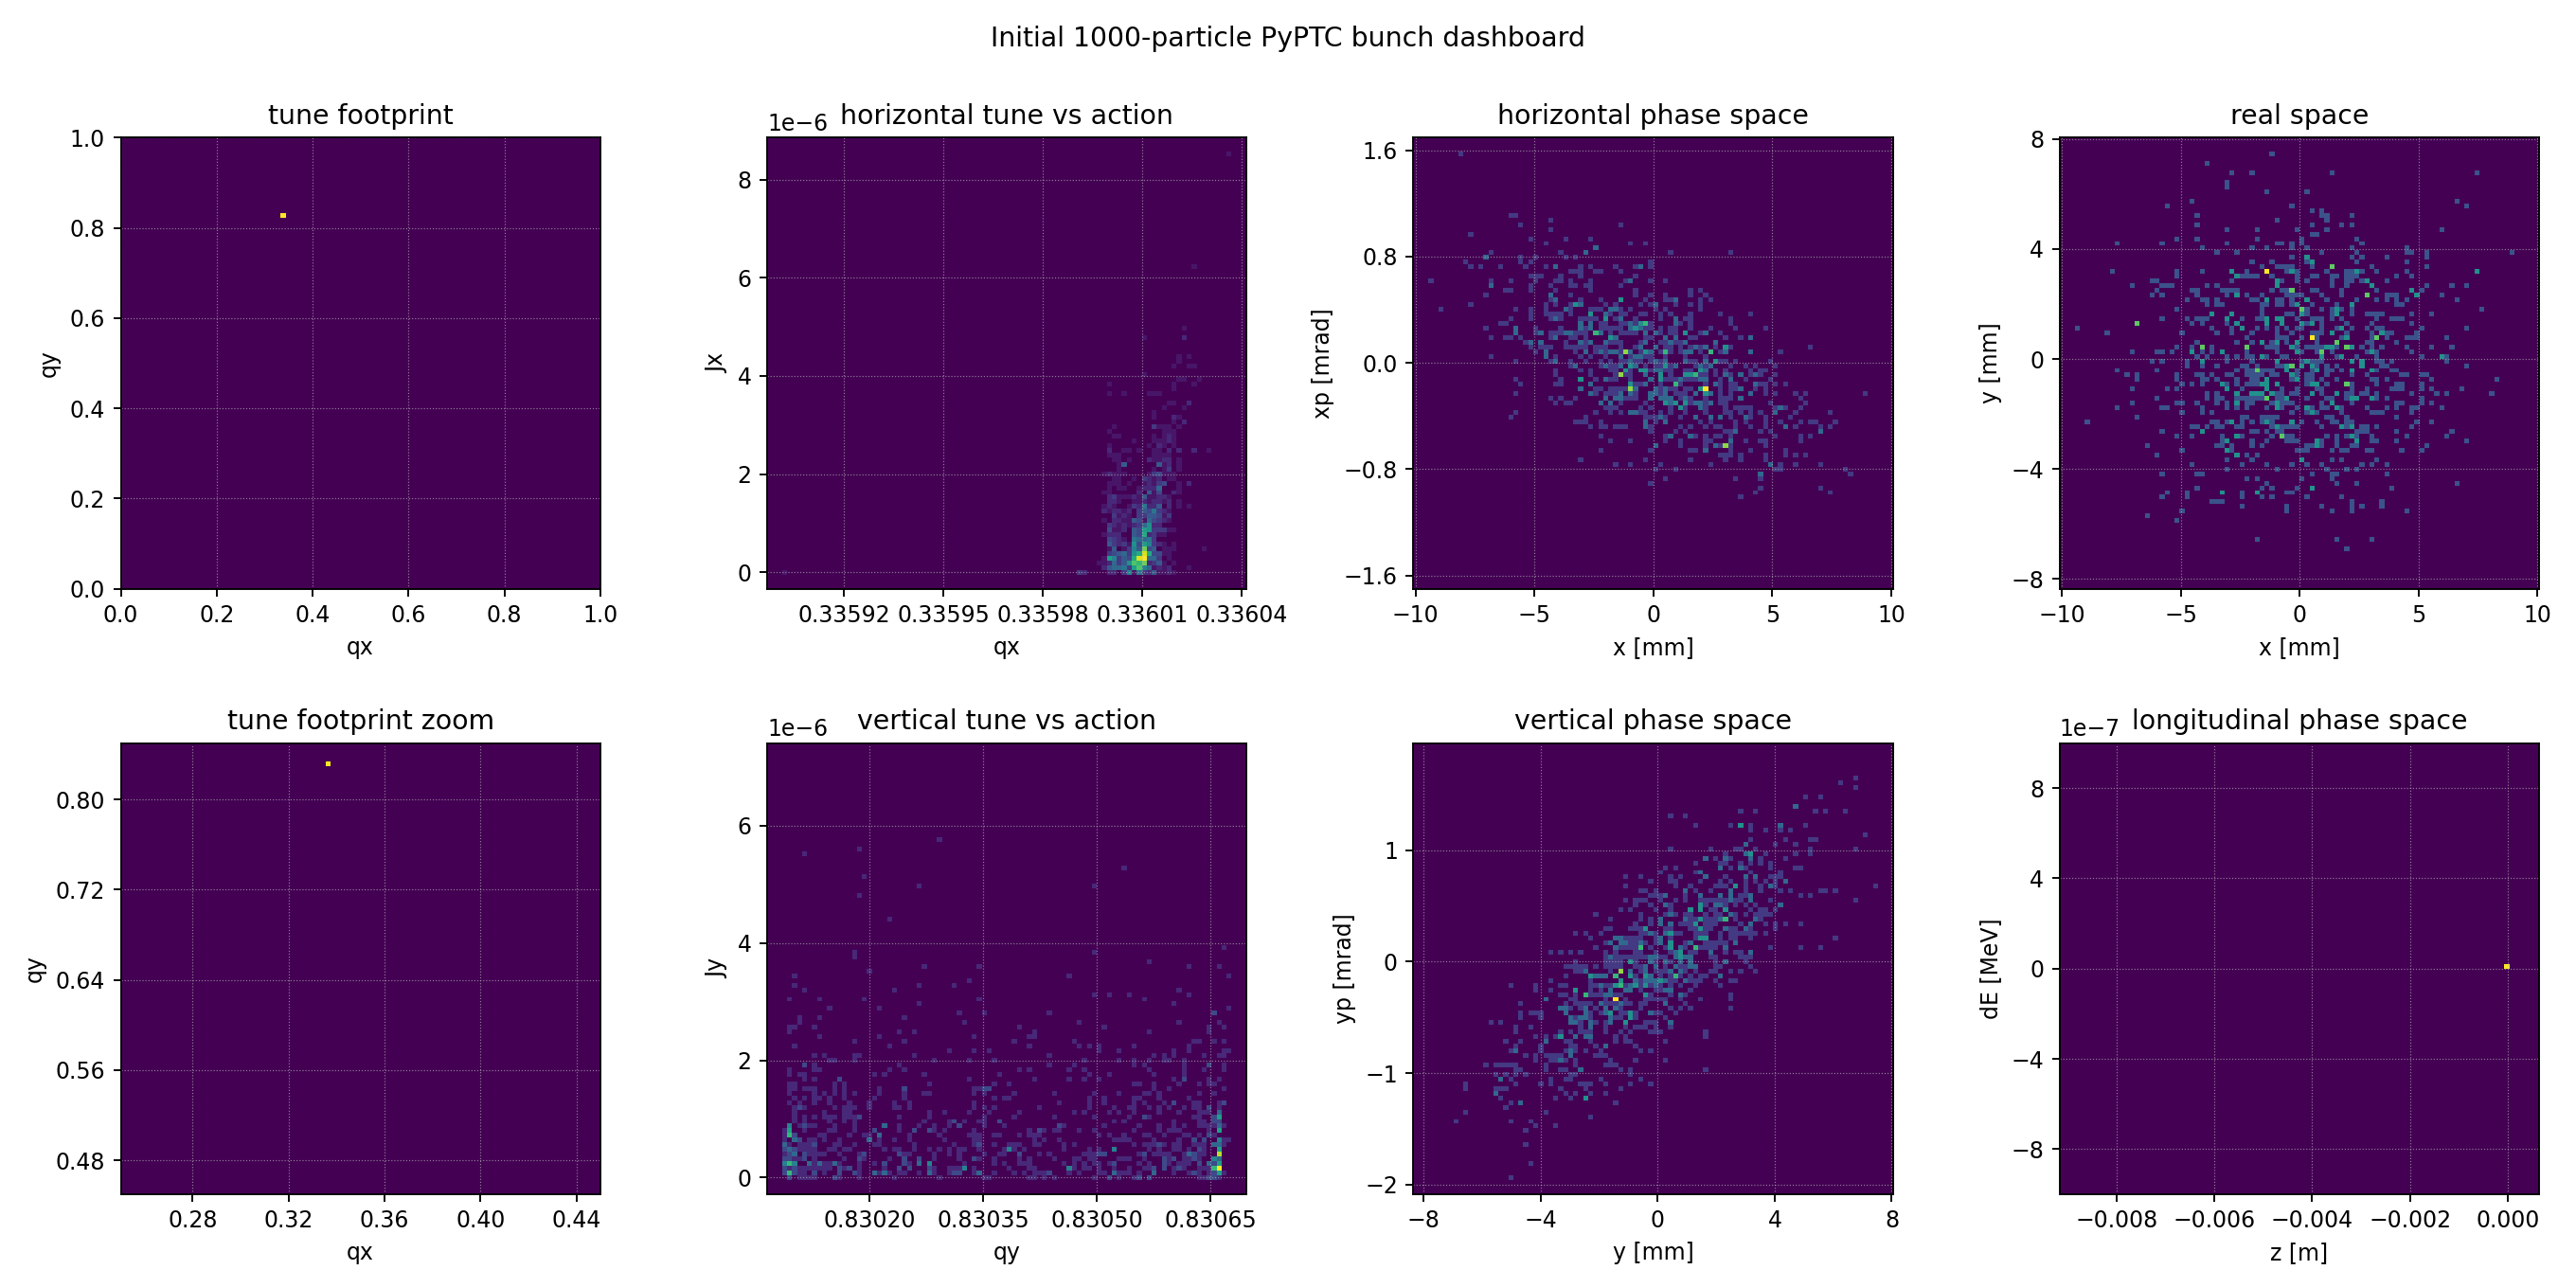
\includegraphics[width=0.88\textwidth]{figures/bunch_initial_dashboard.png}
  \caption{Initial bunch dashboard copied from the standard bunch example output. It records the available diagnostic view before tracking; the associated output directory contains the run summary and diagnostic data. [claim:PROV-03]}
\end{figure}

\begin{figure}[ht]
  \centering
  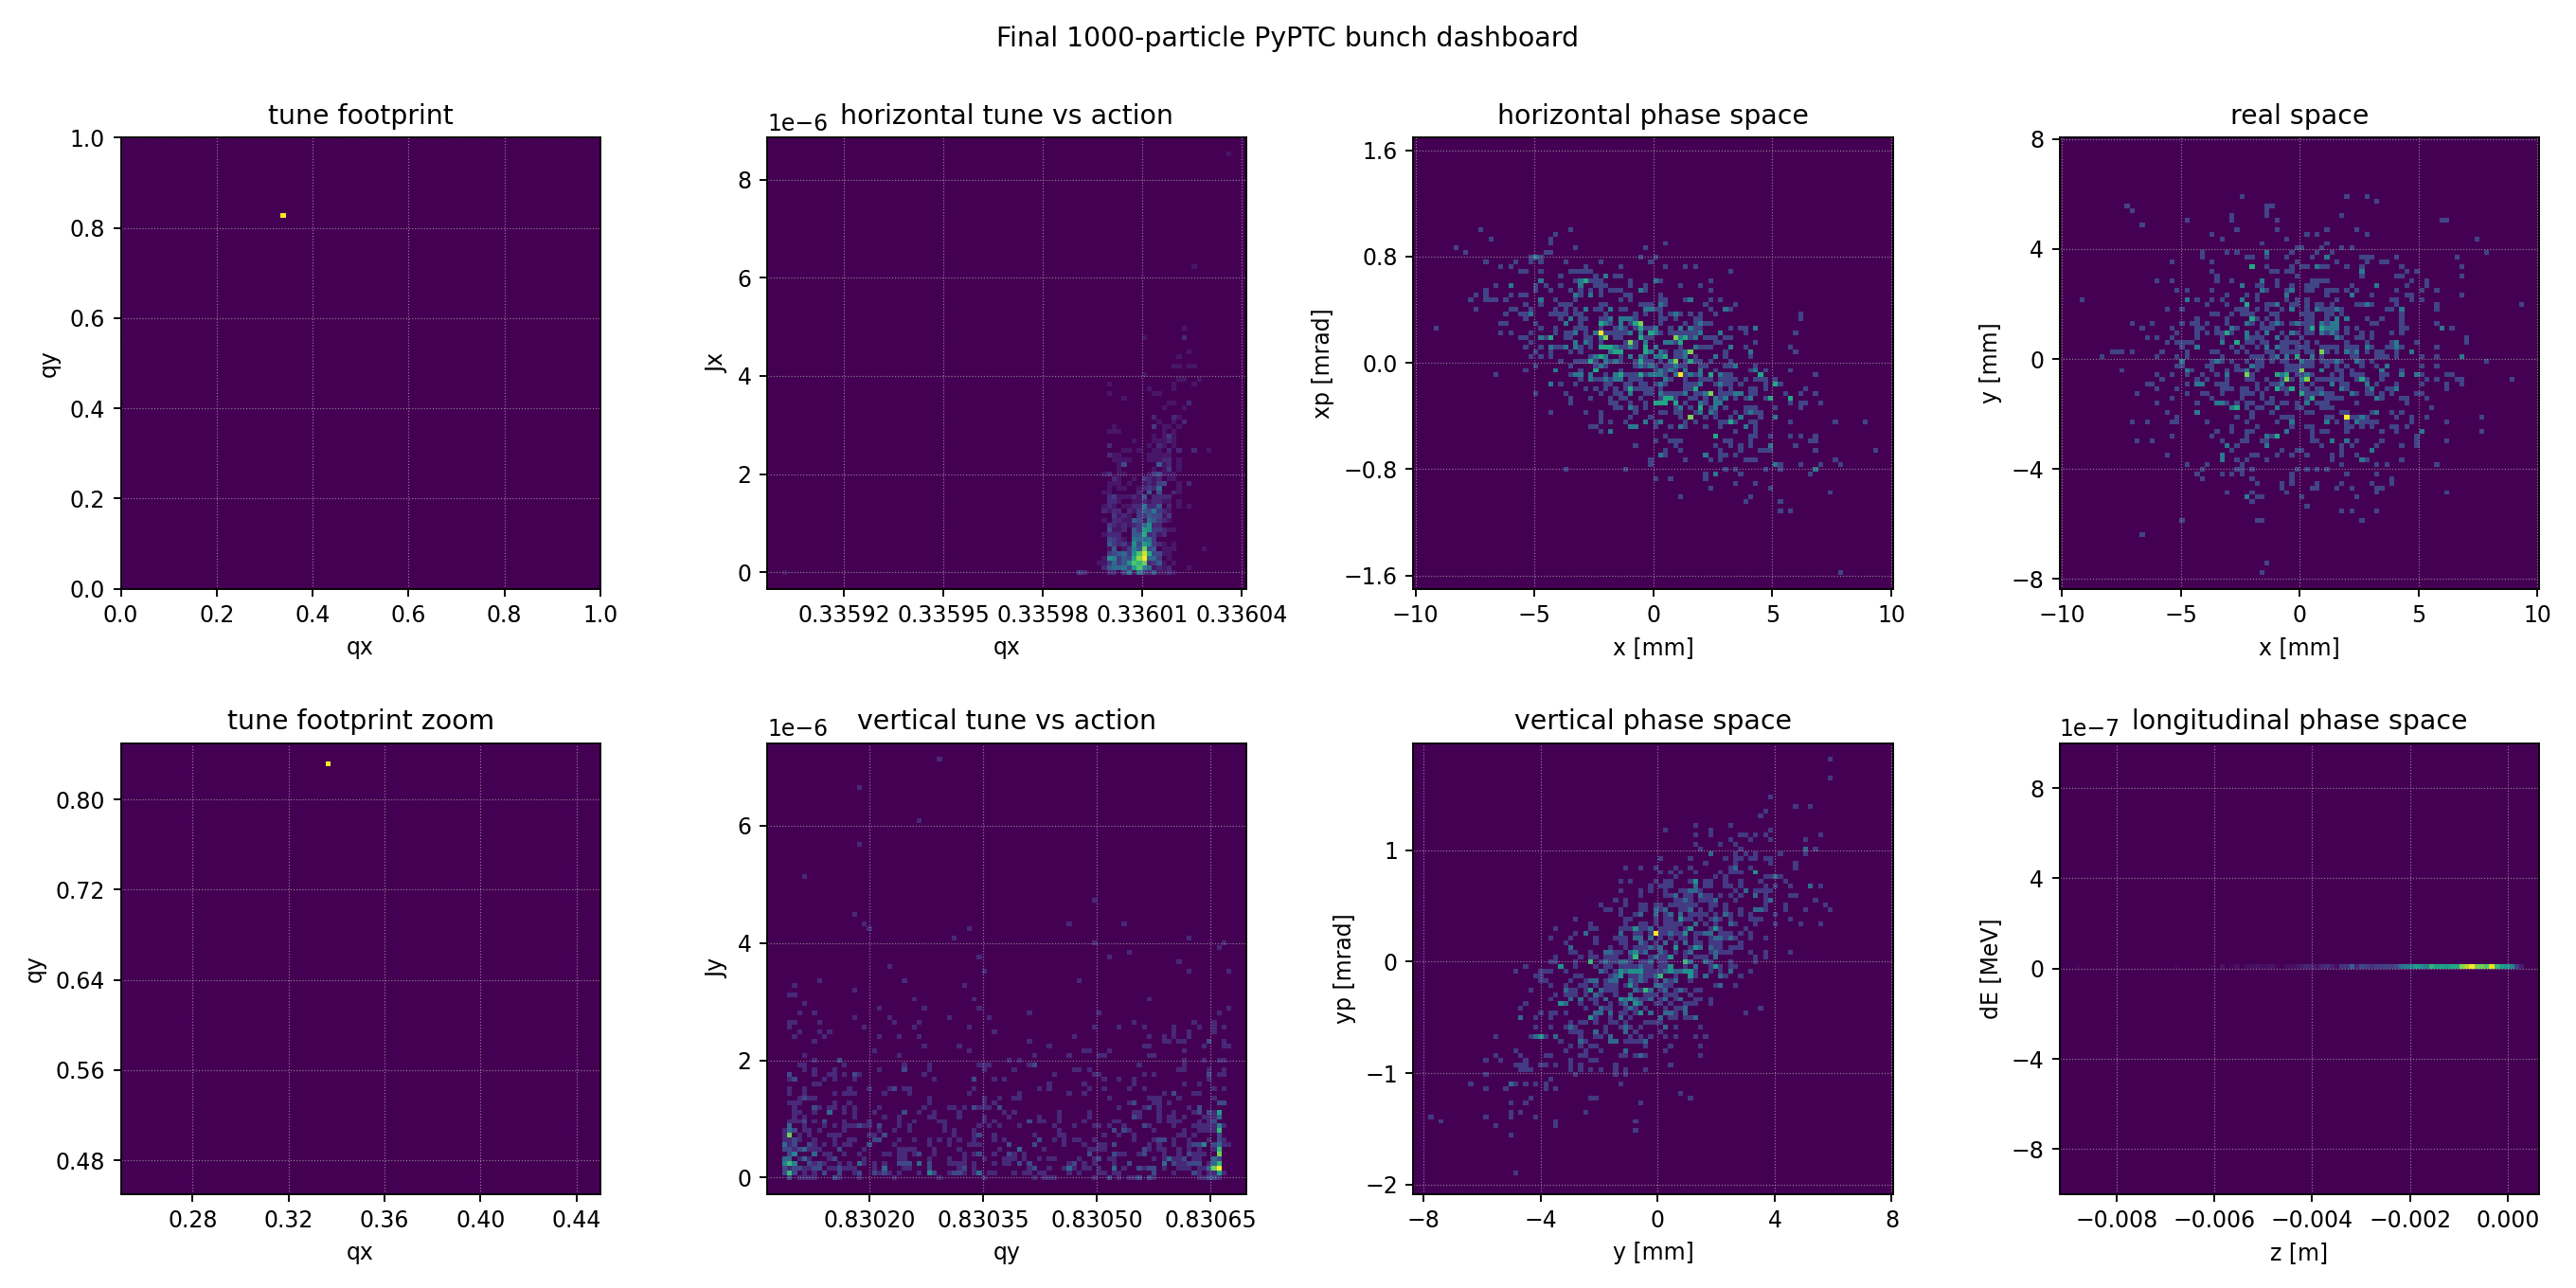
\includegraphics[width=0.88\textwidth]{figures/bunch_final_dashboard.png}
  \caption{Final bunch dashboard from the same example output. Its side-by-side interpretation is limited to this recorded run and the generated input bunch. [claim:PROV-03]}
\end{figure}

\subsection{Apertures and particle loss}

The aperture helpers read rectangular aperture assignments or TFS records, and the JVT CSV reader divides its semi-aperture columns by 1000 before constructing records. The API can apply, query, disable, and set absolute apertures; tracking returns loss flags and loss turn/position fields. The dimensions and operational meaning of input columns should be confirmed by the aperture data owner. [claim:AP-01]

\begin{figure}[ht]
  \centering
  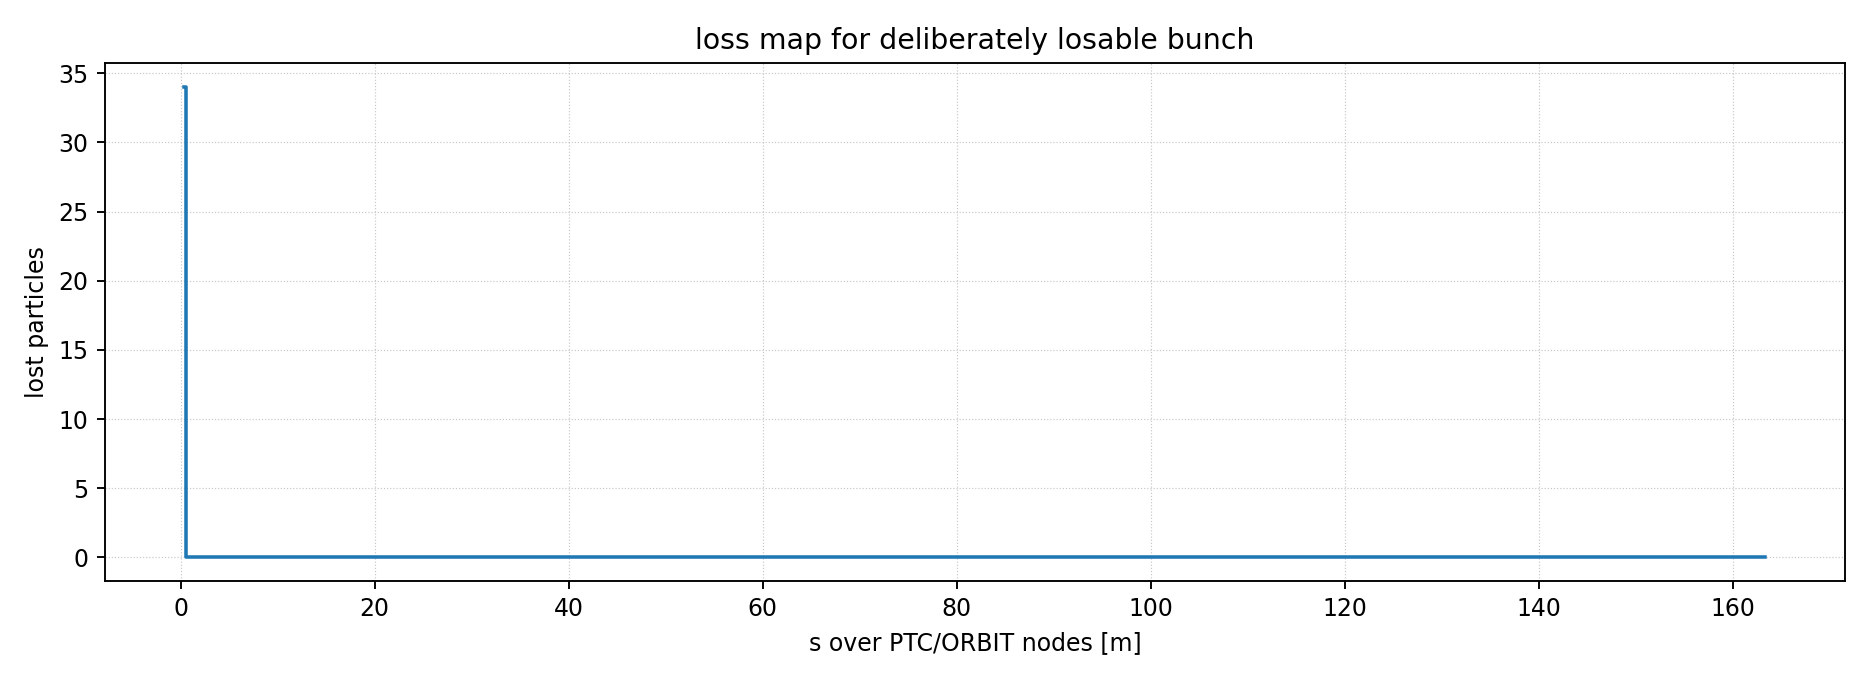
\includegraphics[width=0.82\textwidth]{figures/aperture_loss_map.png}
  \caption{Loss-map image from the aperture example output. It is an example visualization from the stored run and does not establish a validated physical aperture model. [claim:PROV-03] [claim:PROV-04]}
\end{figure}

\section{Lattice edits, errors, and feature boundaries}
\label{sec:edits}

The Python interface exposes element misalignment operations and a parser/application path for MAD-X EFIELD records. The error reader recognizes alignment columns and integrated normal/skew multipole columns through the documented order range. It retains other numeric columns so the caller can reject unsupported nonzero fields instead of silently dropping them. The exact field semantics and units need domain review against the relevant MAD-X/PTC contract. [claim:ERR-01]

The aperture readers and error-table readers are Python-side parsers. They should be treated as converters with explicit supported fields, not as complete MAD-X parsers. Their tests are parser checks; side-by-side example scripts are separate workflow evidence. [claim:API-05]

\begin{center}
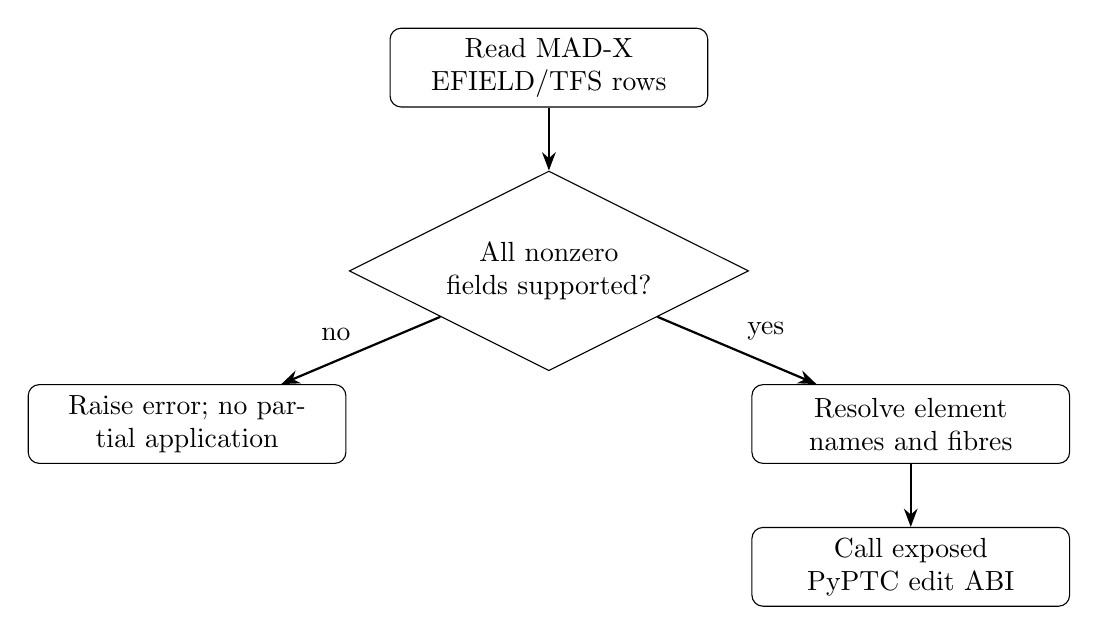
\begin{tikzpicture}[node distance=8mm and 13mm, box/.style={draw,rounded corners,align=center,text width=38mm,minimum height=10mm}, decision/.style={draw,diamond,align=center,aspect=2,text width=29mm}, arr/.style={-{Stealth},thick}]
\node[box] (tfs) {Read MAD-X EFIELD/TFS rows};
\node[decision,below=of tfs] (supported) {All nonzero fields supported?};
\node[box,below left=of supported] (reject) {Raise error; no partial application};
\node[box,below right=of supported] (resolve) {Resolve element names and fibres};
\node[box,below=of resolve] (apply) {Call exposed PyPTC edit ABI};
\draw[arr] (tfs)--(supported);
\draw[arr] (supported)--node[above left]{no}(reject);
\draw[arr] (supported)--node[above right]{yes}(resolve);
\draw[arr] (resolve)--(apply);
\end{tikzpicture}
\end{center}
This diagram represents the wrapper's guarded error-table path. The named interpretation of individual MAD-X fields remains a separate review item. [claim:ERR-01]

\begin{figure}[ht]
  \centering
  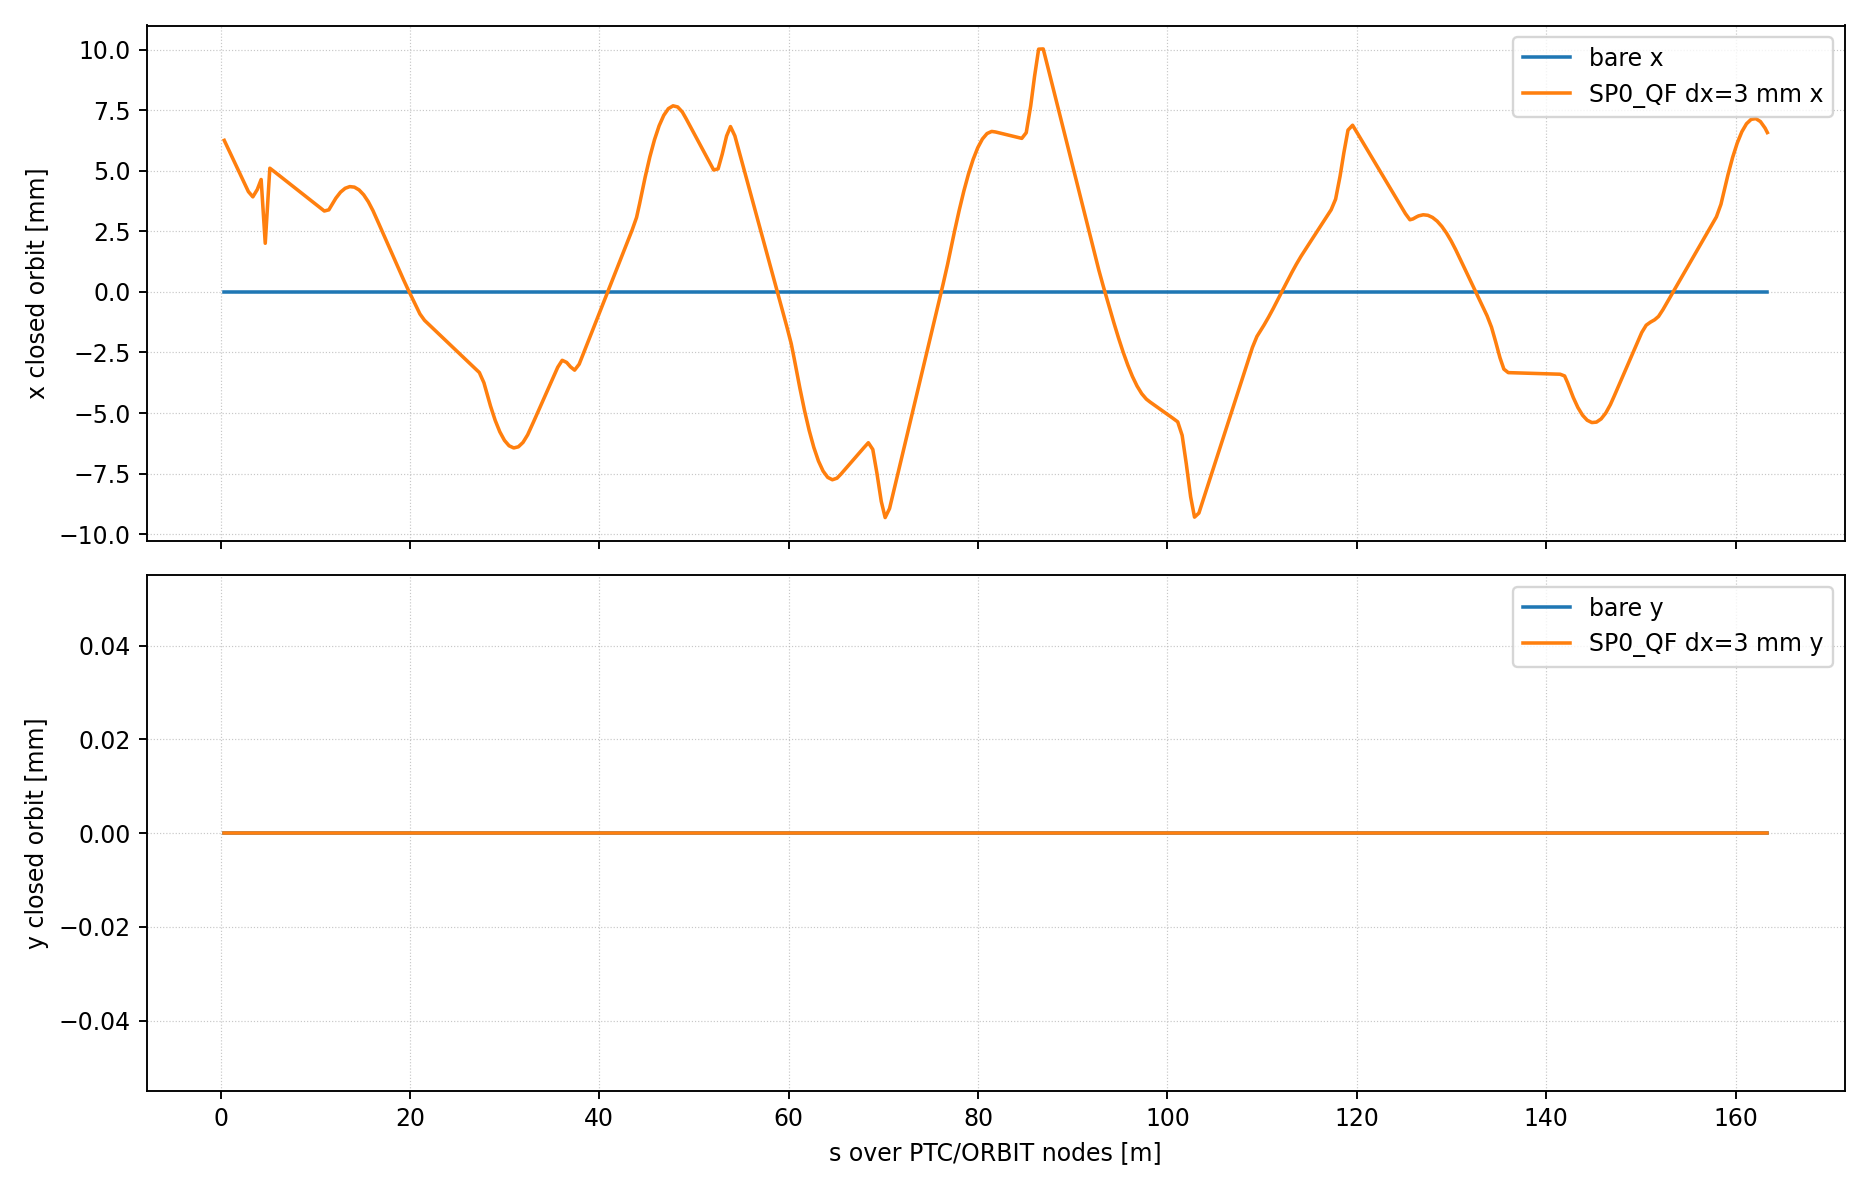
\includegraphics[width=0.84\textwidth]{figures/misalignment_response.png}
  \caption{Single-element misalignment orbit-response plot from the repository example. The example applies a recorded horizontal displacement and compares returned orbit rows. It demonstrates a workflow path, not a machine-calibrated response prediction. [claim:PROV-03] [claim:PROV-04]}
\end{figure}

\begin{figure}[ht]
  \centering
  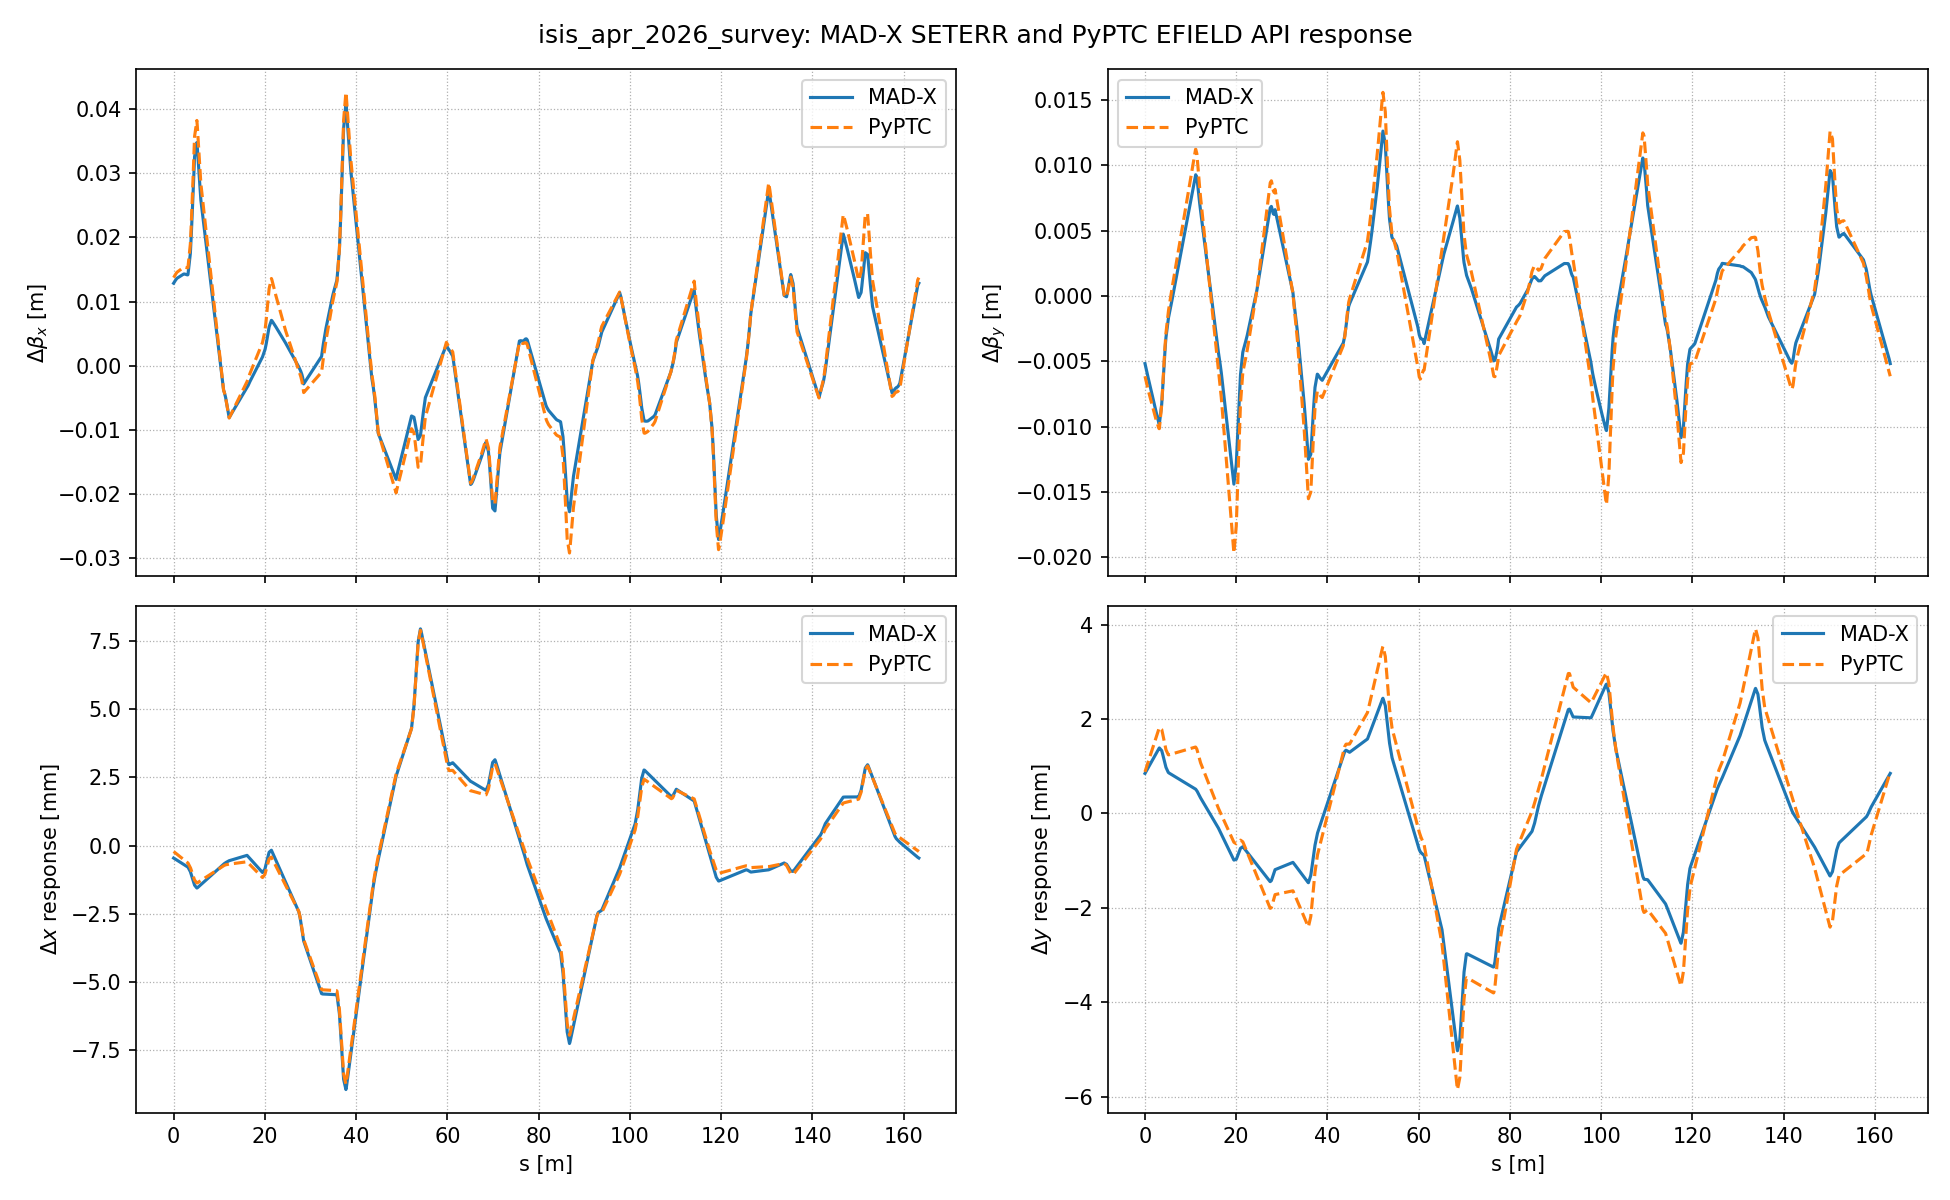
\includegraphics[width=0.88\textwidth]{figures/efield_comparison.png}
  \caption{Stored MAD-X/PyPTC EFIELD side-by-side example for the April 2026 survey table. The companion report records both engines, input and library hashes, and states that the comparison is not tolerance-based acceptance. [claim:PROV-03] [claim:ERR-02] [claim:PROV-04]}
\end{figure}

\begin{figure}[ht]
  \centering
  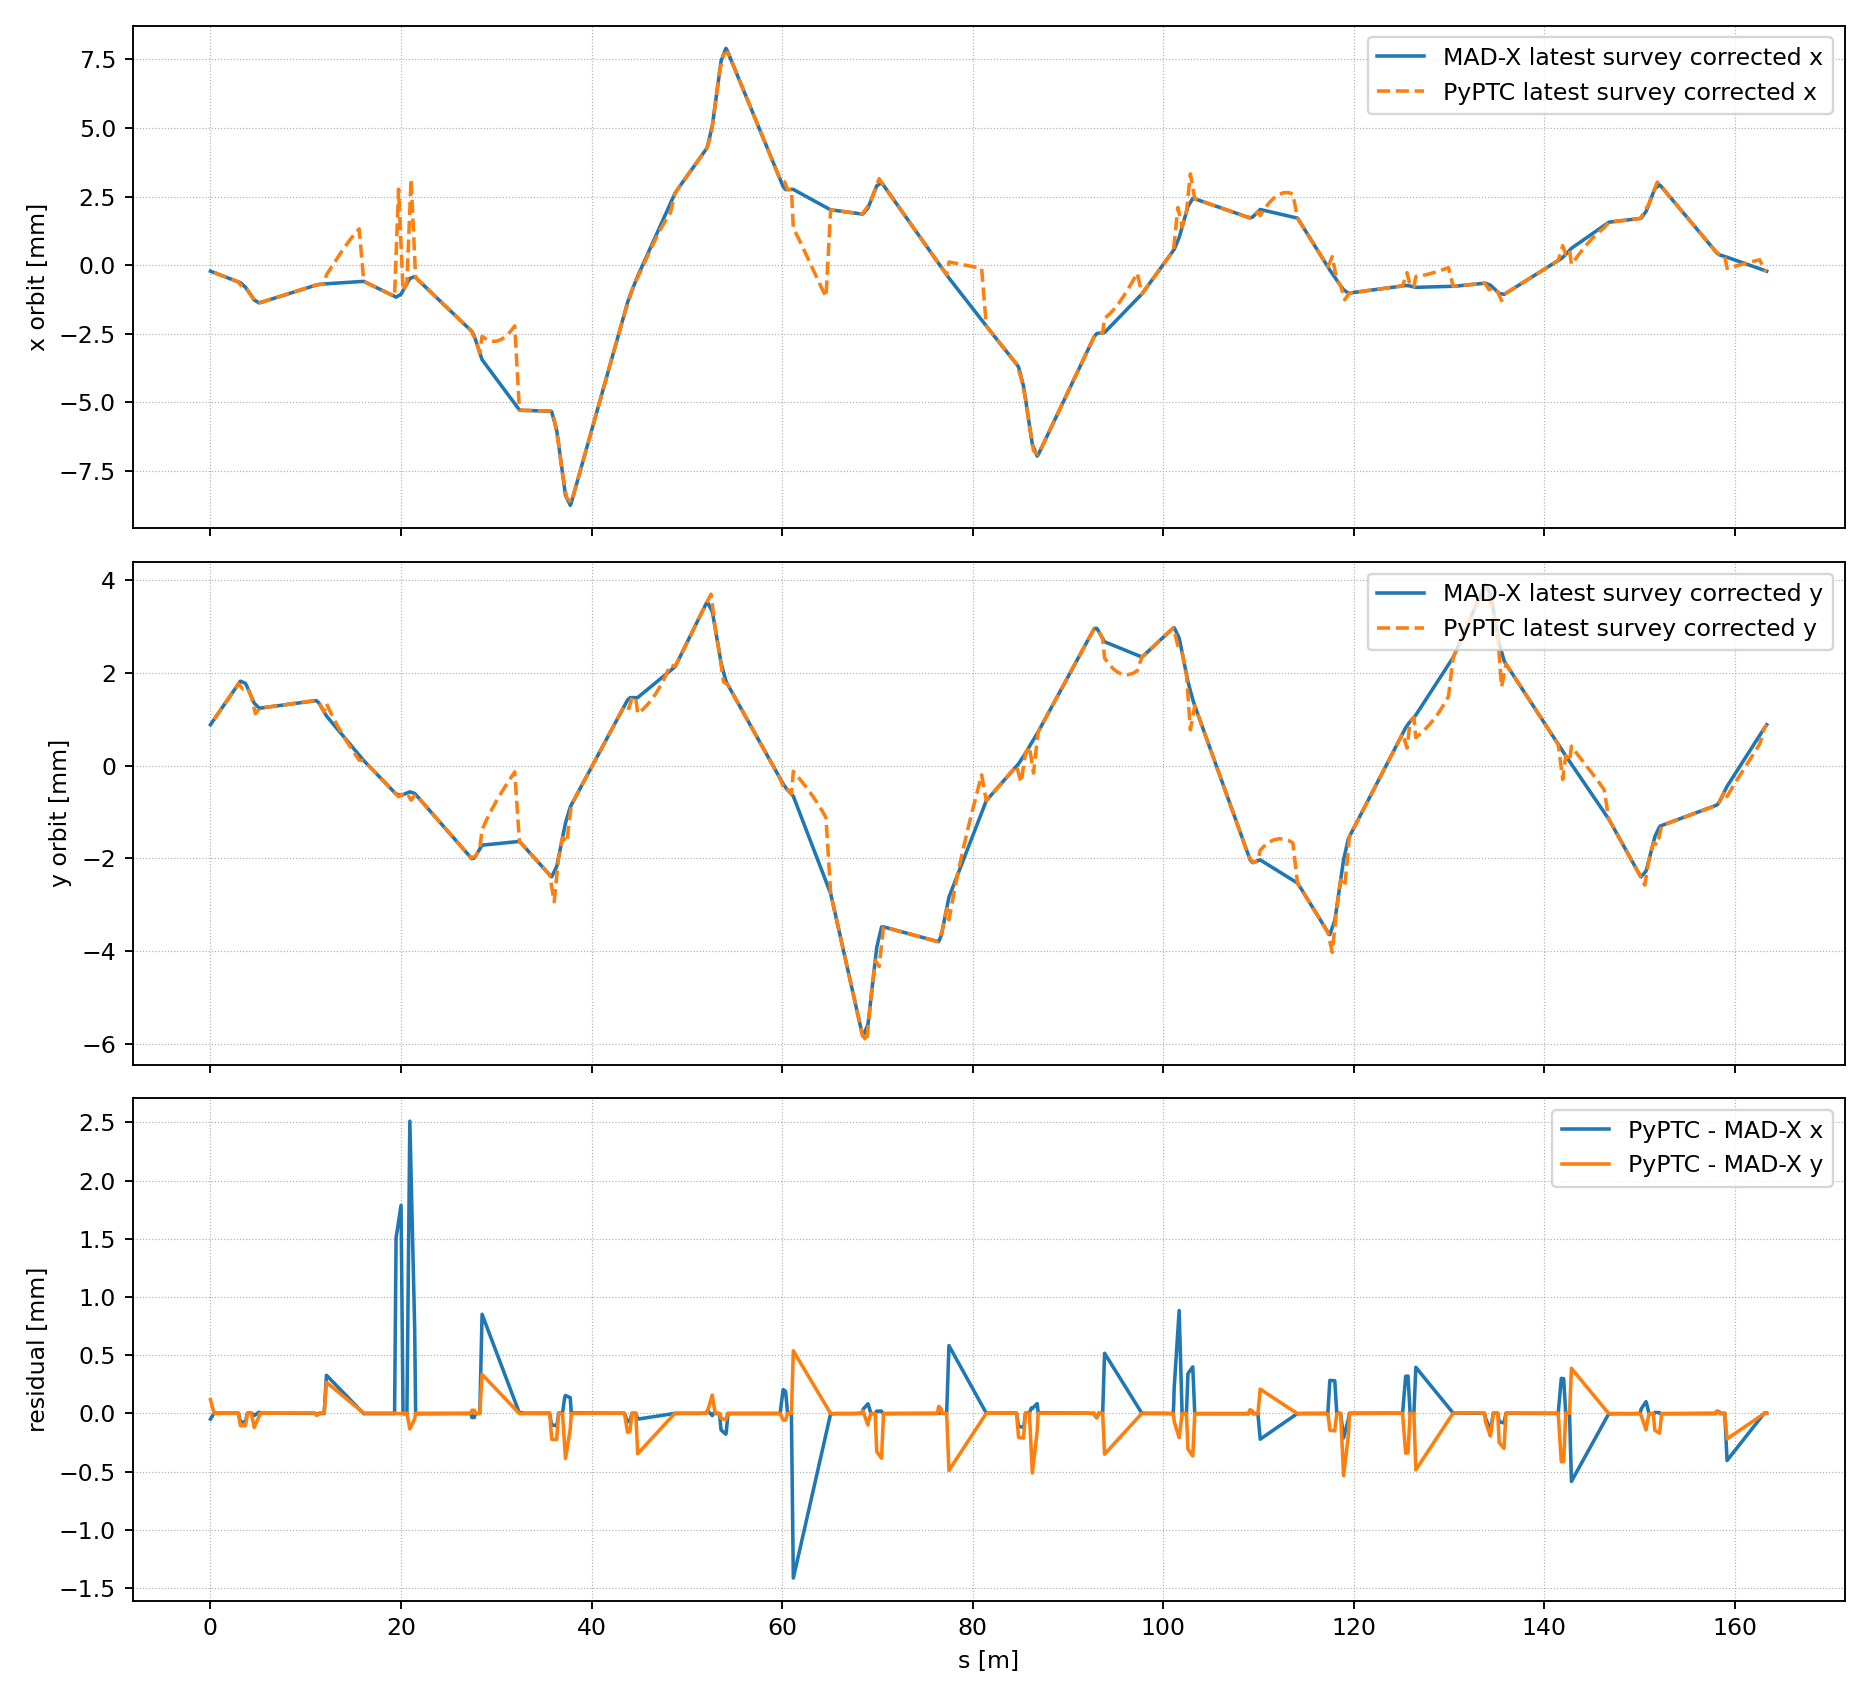
\includegraphics[width=0.88\textwidth]{figures/madx_closed_orbit_comparison.png}
  \caption{Stored full error-table closed-orbit comparison output. This figure belongs to the repository's specific comparison example and its stated table/lattice inputs; it does not define an acceptance tolerance. [claim:PROV-03] [claim:PROV-04]}
\end{figure}

\subsection{Explicitly unexposed paths}

The optics calls \texttt{one\_turn\_map()} and \texttt{normal\_form()} raise a dedicated not-exposed exception. They do not fall back to another calculation. [claim:LIMIT-01]

The normalized-aperture-scan and tune-smear helpers raise the same not-exposed exception. Other PTC features may exist in the underlying library; this guide claims availability only where the repository provides an exposed wrapper path. [claim:LIMIT-02]

\subsection{Examples, tests, and benchmark evidence}

The \texttt{examples/} scripts are runnable demonstrations with user-facing plots and output summaries. \texttt{tests/} contains focused parser and helper checks and separate benchmark-oriented checks. Neither source class should be described as the public API itself. In particular, a MAD-X comparison is evidence for its named case and inputs, not automatic proof of all PyPTC physics behavior. [claim:EXAMPLE-01]

\section{Evidence, limitations, and review status}
\label{sec:evidence}

The figures included in this note are byte-identical copies of repository outputs. The figure manifest gives each source path, hash, command or run context, selection rationale, and the limited claim it supports. Source code hashes, the claim ledger, and literature PDF access status are maintained alongside this note. [claim:PROV-03]

The literature describes broad PTC capabilities, but the current PyPTC wrapper exposes a narrower and versioned subset. This note does not establish validation for an ISIS machine model, acceptance tolerances, or operational use. Existing admission and MAD-X optics benchmark work has its own feedback, ledger, and attempt evidence and must be reviewed through those campaign records. [claim:LIT-01]

\subsection{Unresolved interpretation items}

The following items require named human review before this note can be treated as approved technical guidance:
\begin{itemize}
  \item Python bunch coordinates versus the internal PTC coordinate slots, including units, signs, and longitudinal scaling. [claim:TRACK-02]
  \item The meaning and unit convention of returned Twiss, orbit, chromaticity, and phase fields. [claim:PHYS-01]
  \item MAD-X EFIELD alignment/multipole unit and sign mapping at the PyPTC boundary. [claim:ERR-02]
  \item Which repository examples and benchmark cases are suitable as approved golden cases. [claim:PROV-04]
\end{itemize}

\subsection{Review gates}

Code correspondence: pending. Physics interpretation: pending. Reader usefulness: pending. No agent has marked any claim reviewed. A future reviewer should be named in \texttt{CLAIMS.toml}, answer the acceptance questions in the evidence skill, and record the review date and disposition. [claim:PROV-02]

\subsection{Reproducibility record}

The source manifest records the checked-out commit and hashes. The quick-start build command is \texttt{bash build/build\_ptc.sh}; the note itself is built from this directory with \texttt{pdflatex} and \texttt{bibtex}. The execution log, exact commands, result, PDF hash, and page-inspection notes are recorded in \texttt{PLAN.md}. Drafting used an AI assistant with human review pending. [claim:PROV-01]


\section{References}
\nocite{ForestSchmidtMcIntosh2002,ForestNogiwaSchmidt2006FPPPTC,ForestNogiwaSchmidt2006FPPDoc,Schmidt2005MADXPTC,SkowronskiSchmidtForest2007,MADXPTCManual2006,ForestSchmidtPTCManual2010,Forest2016Tracking}
\bibliographystyle{plain}
\bibliography{../references}
\end{document}
